\section{Propagación en medios elásticos}
\label{sec:fundamentos}

Un impacto aplicado sobre la superficie altera localmente el estado de equilibrio del suelo. Esa perturbación se transmite, pues cada elemento material ejerce fuerzas sobre sus vecinos. Para relacionar la respuesta observada con las características del terreno es necesario comprender tal comportamiento mecánico y distinguir las formas de movimiento que admite un medio elástico.

\subsection{Ondas de cuerpo en un medio elástico}
\label{sec:medio-elastico}

En el régimen de pequeñas deformaciones, la estructura granular del suelo se sustituye por un medio continuo: cada volumen elemental agrupa un gran número de partículas y sus propiedades representan el comportamiento conjunto. Bajo las hipótesis iniciales de homogeneidad e isotropía, su respuesta puede describirse paramétricamente mediante la densidad $\rho$ y los parámetros de Lamé $\lambda$ y $\mu$. La densidad gobierna la inercia; $\lambda$ participa en la oposición al cambio de volumen, y $\mu$ es el módulo de corte que cuantifica la oposición al cambio de forma. Si $\mathbf{u}(\mathbf{x},t)$ es el desplazamiento, el equilibrio lineal queda expresado por \citep{Kramer1996,Foti2014}
\begin{equation}
\rho\,\frac{\partial^2\mathbf{u}}{\partial t^2}
=(\lambda+\mu)\nabla(\nabla\!\cdot\!\mathbf{u})+
\mu\nabla^2\mathbf{u}.
\label{eq:navier}
\end{equation}
Esta idealización permite reconocer de primera mano los mecanismos elementales de propagación.

La aceleración de cada volumen elemental puede provenir de una deformación volumétrica o de corte. La descomposición de Helmholtz separa ambos movimientos mediante un potencial escalar $\phi$ y uno vectorial $\mathbf{\Psi}$ \citep{Foti2014}:
\begin{equation}
\mathbf{u}=\nabla\phi+\nabla\times\mathbf{\Psi},
\qquad \nabla\cdot\mathbf{\Psi}=0.
\label{eq:helmholtz}
\end{equation}
Al sustituirla en la ecuación~\eqref{eq:navier} aparecen dos soluciones independientes. La primera produce compresiones y dilataciones en la dirección de avance y se denomina onda P, inicial asociada en inglés con \emph{primary} y \emph{pressure}. La segunda produce deformación transversal de corte y se denomina onda S, por \emph{secondary} y \emph{shear}. Sin introducir aún una fuente concreta, estas soluciones muestran que un mismo material admite dos formas de transportar una perturbación.

Las velocidades de propagación correspondientes son
\begin{equation}
V_P=\sqrt{\frac{\lambda+2\mu}{\rho}},
\qquad
V_S=\sqrt{\frac{\mu}{\rho}}.
\label{eq:velocidades}
\end{equation}
Un receptor permanece en una localización fija y observa la oscilación local cuando el frente de onda pasa por ella. La figura~\ref{fig:ondas-ps} muestra la diferencia entre el movimiento longitudinal P y el transversal S.

\begin{figure}[!tb]
\centering
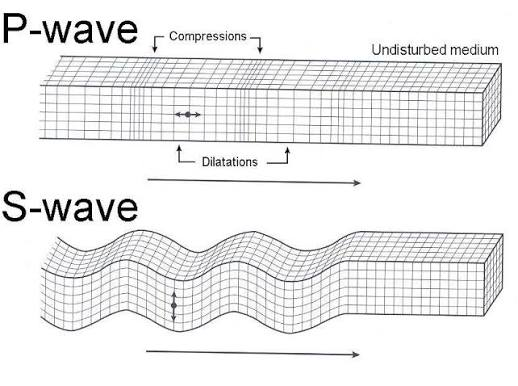
\includegraphics[width=0.98\columnwidth]{fig01_ondas_p_s.png}
\caption{Deformación y movimiento local asociados con ondas P y S. En P las partículas oscilan paralelamente al avance; en S lo hacen en dirección transversal. Adaptada de \citet{Kearey2002}, a partir de Bolt.}
\label{fig:ondas-ps}
\end{figure}

La segunda relación de la ecuación~\eqref{eq:velocidades} conduce a
\begin{equation}
G_{\max}=\rho V_S^2,
\label{eq:rigidez}
\end{equation}
donde $G_{\max}$ es el módulo de corte a pequeñas deformaciones. Esta vinculación es de gran interés geotécnico, pues la propagación de las ondas S aporta información sobre la rigidez inicial del suelo cuando se dispone de una estimación de densidad \citep{Kramer1996,Foti2014}. La misma magnitud es la que miden los ensayos \emph{downhole} y \emph{crosshole}, de modo que los métodos de superficie y los invasivos pueden contrastarse mutuamente: la medición en pozo calibra la interpretación superficial y ésta extiende a todo el tramo lo observado en el pozo. Tal estimación no reemplaza los parámetros de diseño bajo cargas mayores: este modelo lineal no incorpora disipación energética ni el comportamiento plástico del material.

\subsection{Interfaces y conversión de modos}

Las ondas S admiten dos polarizaciones. La componente SV se mueve dentro del plano vertical de propagación, mientras que la componente SH lo hace horizontalmente y perpendicular a ese plano. Esta distinción se vuelve relevante al alcanzar las condiciones de frontera del material. Puede encontrarse el contacto con otro material o una superficie libre; en ambos casos se hablará de una interfaz.

Cuando una componente P o SV incide oblicuamente sobre el contacto entre dos sólidos, los contrastes de densidad y rigidez reparten su energía entre ondas reflejadas y transmitidas y permiten conversión P--SV, como resume la figura~\ref{fig:conversion-interfaz}. La componente SH permanece desacoplada de P y SV en una interfaz plana entre medios elásticos isótropos: sólo produce componentes SH reflejadas y transmitidas \citep{Foti2014,Sun2003}.

\begin{figure}[!tb]
\centering
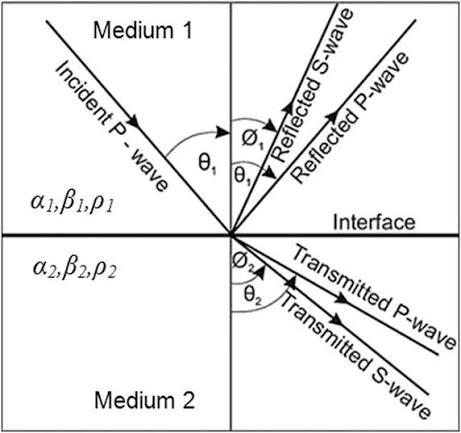
\includegraphics[width=0.80\columnwidth]{fig02_conversion_interfaz.png}
\caption{Reflexión, transmisión y conversión P--SV de una onda P al alcanzar una interfaz entre dos medios elásticos. Adaptada de \citet{Bangash2017}.}
\label{fig:conversion-interfaz}
\end{figure}

El límite superior del terreno es una interfaz particular. El aire, al igual que el agua, es un fluido y no puede sostener esfuerzos de corte, por lo que ninguno de los dos transmite ondas S; en la superficie libre deben satisfacerse condiciones de tensión nula.

\subsection{Ondas superficiales}
\label{sec:rayleigh}

En la superficie libre las componentes reflejadas interactúan y aparecen soluciones cuya energía permanece principalmente en la zona somera; se denominan ondas superficiales. Según las ondas de cuerpo que las conforman se distinguen dos familias. El movimiento SH guiado por las capas da origen a las ondas Love, cuyas partículas se desplazan horizontalmente y en dirección transversal a la propagación. Las componentes P y SV, en cambio, se acoplan en la superficie y producen la onda Rayleigh, cuyas partículas describen trayectorias elípticas en el plano vertical, semejantes a las de las olas en el agua pero recorridas en la superficie en sentido retrógrado respecto de la propagación \citep{Foti2014,Foti2018}.

En un semiespacio homogéneo con propiedades habituales del suelo, la velocidad de fase de la onda Rayleigh es sólo ligeramente menor que $V_S$. Por ello, su medición es una vía indirecta y no invasiva hacia la rigidez de la ecuación~\eqref{eq:rigidez}. Además, su movimiento vertical puede excitarse con un golpe sobre la superficie y observarse con un único transductor vertical; por esta razón el proyecto se concentra en ondas Rayleigh y no en Love.

La expansión geométrica también favorece su observación a cierta distancia de la fuente. En condiciones ideales de campo lejano, la amplitud de las ondas de cuerpo se reduce aproximadamente como $r^{-1}$ al distribuirse sobre un frente esférico, mientras que la de las ondas superficiales lo hace como $r^{-1/2}$ sobre un frente cilíndrico. Por esta menor tasa de decaimiento, las componentes Rayleigh suelen dominar el registro superficial \citep{Foti2014}.

\subsection{Estratificación y dispersión}
\label{sec:dispersion}

En un semiespacio homogéneo, un modo Rayleigh conserva la misma velocidad de fase para todas las frecuencias. El suelo real, en cambio, está estratificado. Las componentes de menor frecuencia y mayor longitud de onda involucran un volumen más profundo, mientras que las de mayor frecuencia se concentran cerca de la superficie. Como cada una pondera una combinación diferente de capas, avanzan con velocidades de fase distintas. Esta dependencia con la frecuencia se denomina dispersión \citep{Foti2014,Foti2018}. La relación
\begin{equation}
\lambda_R(f)=\frac{c_R(f)}{f}
\label{eq:longitud-onda}
\end{equation}
vincula longitud de onda $\lambda_R$, frecuencia $f$ y velocidad de fase $c_R$. No asigna una profundidad única a cada frecuencia, pero muestra por qué una longitud de onda mayor interroga una región más extensa. La figura~\ref{fig:rayleigh-frecuencia} ilustra esta diferencia de alcance en un medio de tres capas.

\begin{figure}[!tb]
\centering
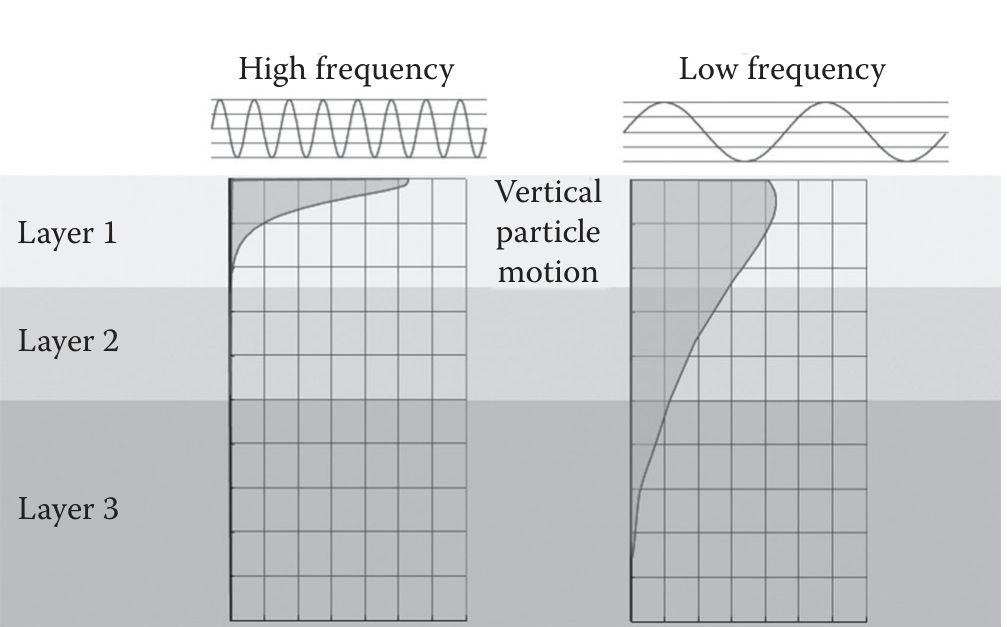
\includegraphics[width=0.98\columnwidth]{fig03_foti_dispersion_profundidad.png}
\caption{Movimiento vertical de las partículas en función de la profundidad para una onda Rayleigh de alta y de baja frecuencia en un medio de tres capas. Adaptada de \citet{Foti2014}.}
\label{fig:rayleigh-frecuencia}
\end{figure}

En consecuencia, resulta de interés obtener la evolución temporal y espacial de la señal para comparar el avance de cada componente frecuencial. Al observar cómo cambia la señal con la frecuencia y la posición puede construirse posteriormente un modelo compatible con la variación de rigidez. Esta necesidad conduce de manera natural a los métodos de análisis de ondas Rayleigh.
